\documentclass[12pt,a4paper,oneside]{article}
\usepackage[colorlinks=true, unicode]{hyperref}
\usepackage[utf8]{inputenc}
\usepackage[czech]{babel}
\usepackage{graphicx}
\usepackage{pdfpages}
\textwidth 16cm \textheight 25cm
\topmargin -1.3cm 
\oddsidemargin 0cm
\usepackage{footnote}
\pagestyle{empty}
\begin{document}
\title{Základní RF zesilovač - GB01A}
\author{Jakub Kákona, kaklik@mlab.cz}
\maketitle

\thispagestyle{empty}
\begin{abstract}
Poskytuje širokopásmový zisk závislý podle osazeného MMIC obvodu.
\end{abstract}

\begin{figure} [htbp]
\begin{center}
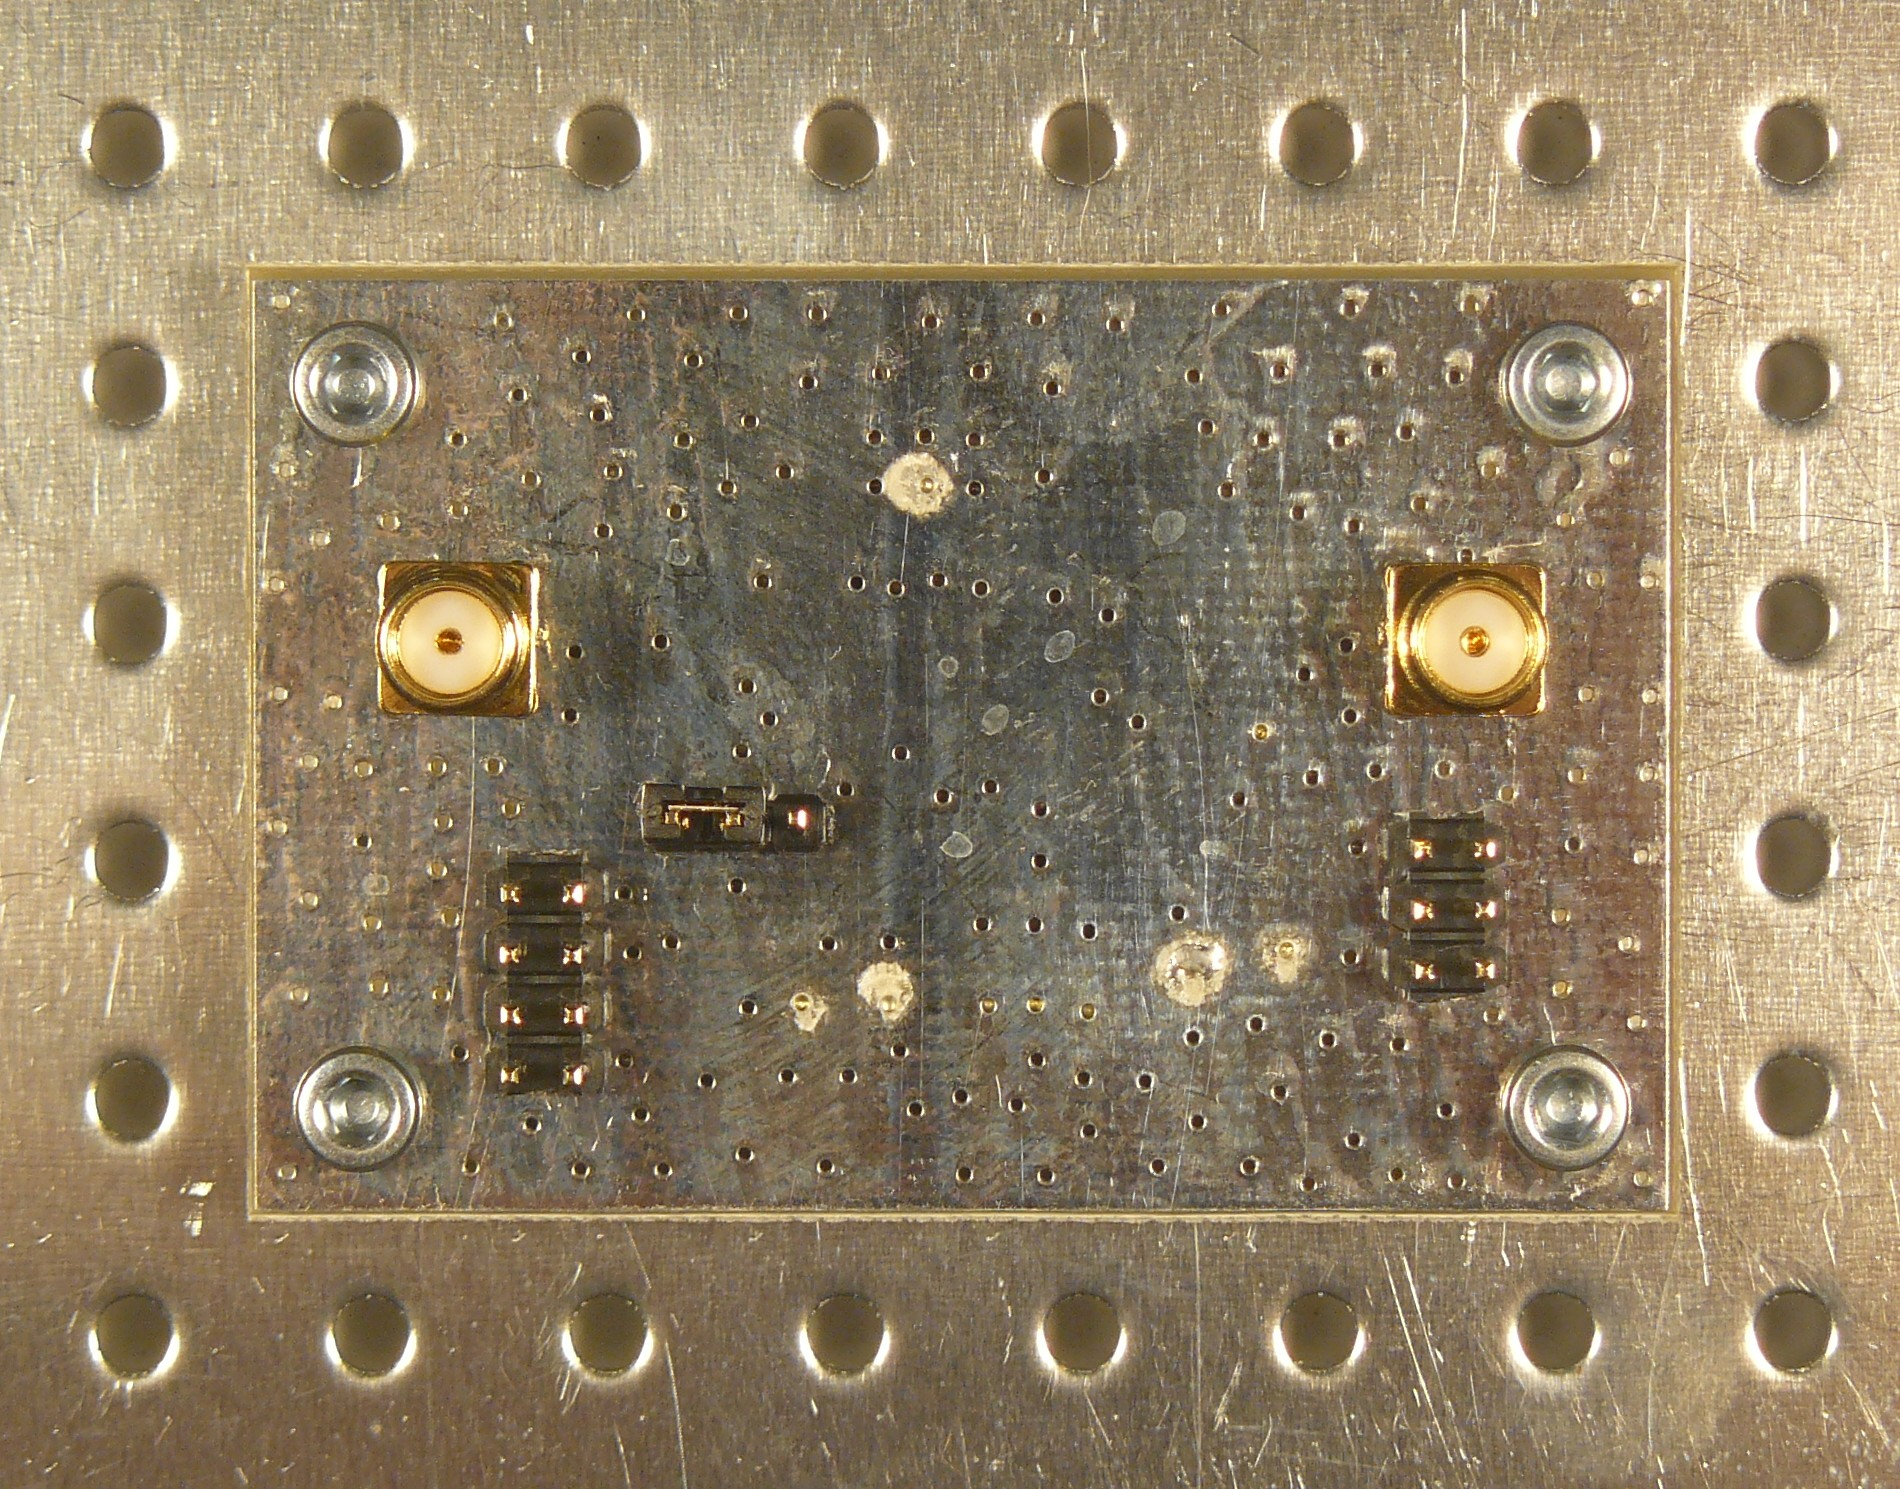
\includegraphics [width=80mm] {./img/GB01A_Top_Big.JPG} 
\end{center}
\end{figure}

\begin{figure} [b]

\includegraphics [width=25mm] {./img/GB01A_QRcode.png} 
\end{figure}

\newpage
\tableofcontents

\section{Technické parametry}
\begin{table}[htbp]
\begin{center}
\begin{tabular}{|c|c|p{4.7cm}|}
\hline
Parametr & Hodnota & Poznámka \\
\hline
Napájecí napětí POWER  & max 5V &  160mA \\ 
\hline
Napájecí napětí Vcore & +1,8V, 2,7V, 3,3V &  Záleží na konkrétním typu čipu Si5XX \\ 
\hline
Frekvenční rozsah  & 10 - 1500 MHz & Záleží na konkrétním typu čipu Si5XX, obvykle 10-810MHz \\ 
\hline
Fázový jitter  & $<$ 0,3ps & Pro obvody řady Si570 \\ 
\hline
\end{tabular}
\end{center}
\end{table}

\section{Popis konstrukce}

\subsection{Zapojení}
Zapojení modulu je řešeno tak, aby umožnilo připojení řídícího mikroprocesoru provozovaného na stejném i jiném napájecím napětí vůči čipu Si5XX. V konstrukci je proto využit převodník napěťových úrovní, který může být při jeho absenci přemostěn dvěma nulovými odpory R4 a R5.

V případě provozování modulu na napájecím napětí různém od napájecího napětí Si570 si modul může stabilizovat napájení sám díky lineárnímu stabilizátoru. V takovém případě je ale přesto dát pozor, aby napájení nepřesáhlo dovolené napětí na translátoru, tedy hranici 5V. 

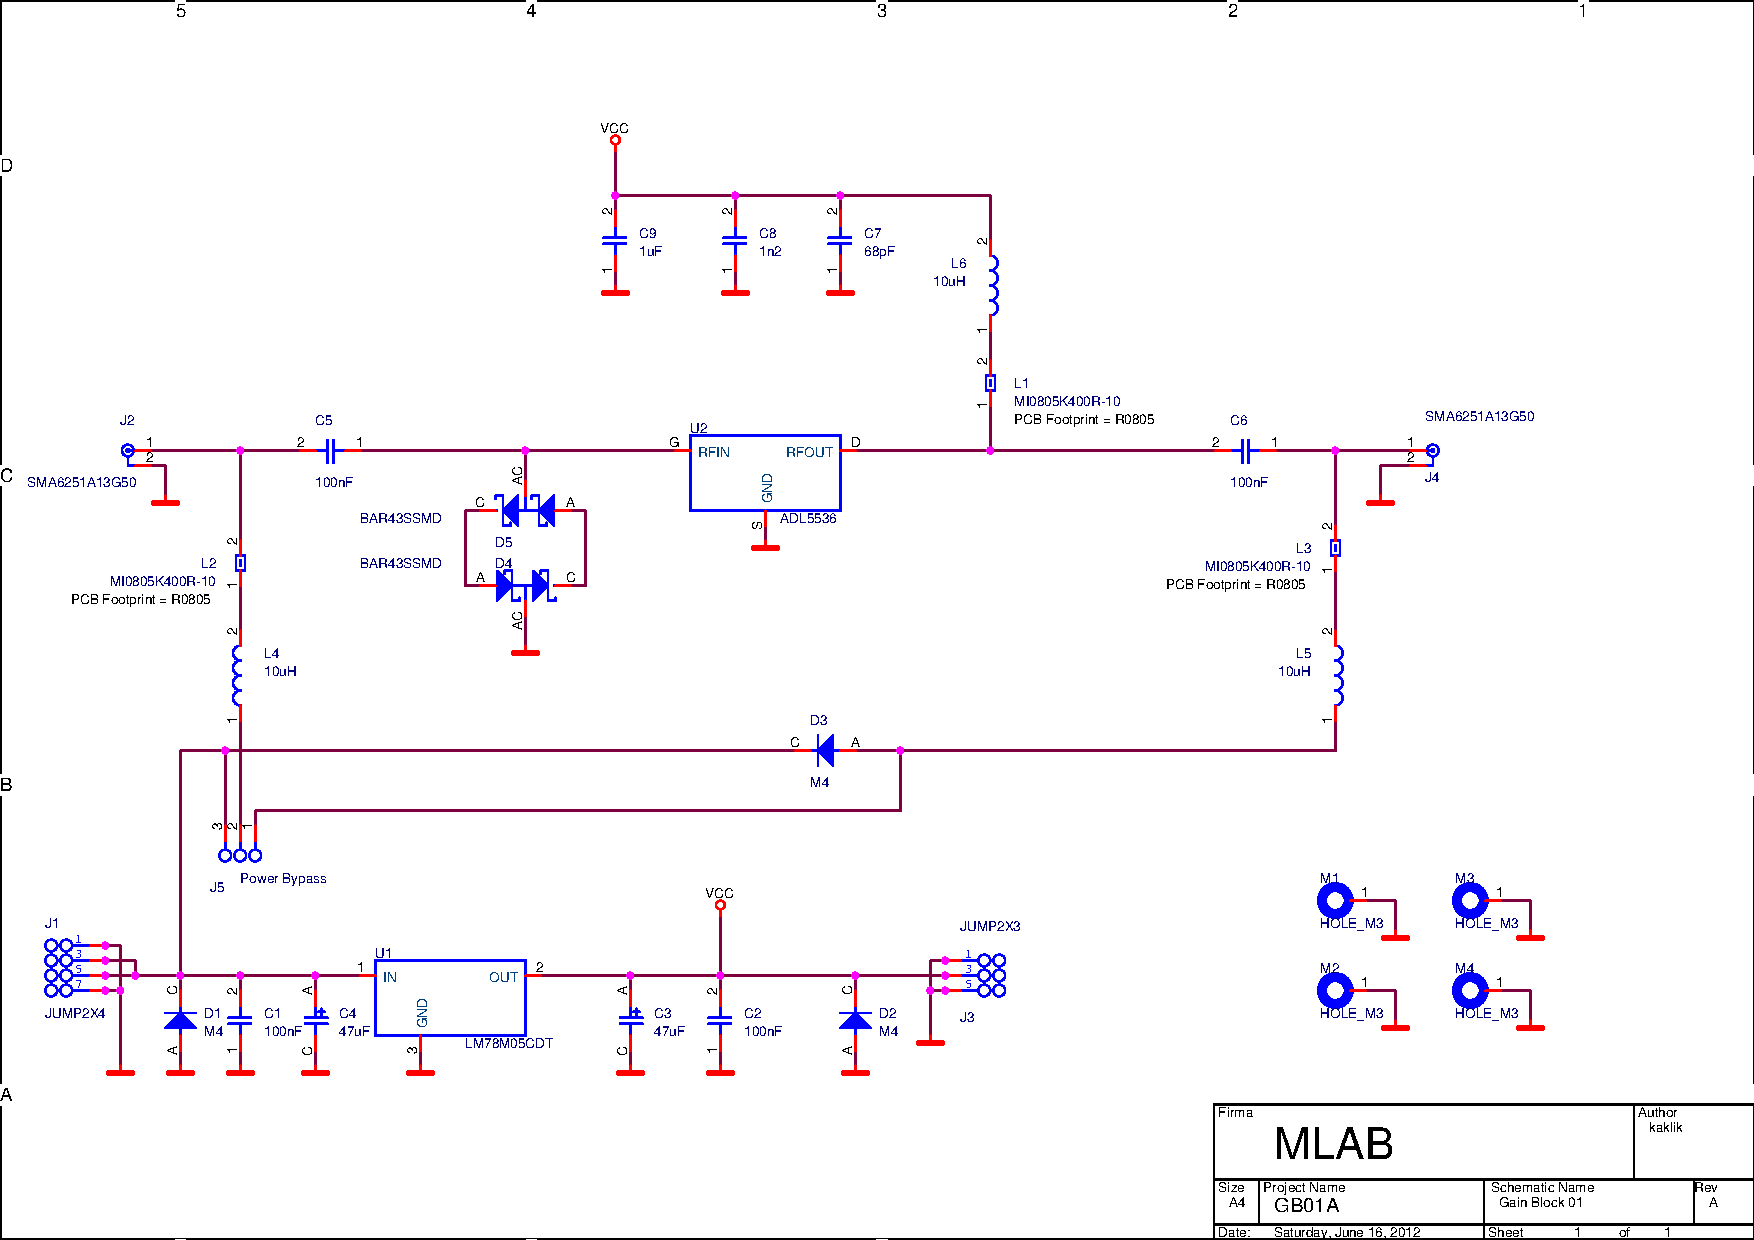
\includepdf[pages={1},landscape=true]{../../SCH/GB01A.pdf}

Jak je vidět ze zapojení, výstup je předpokládán diferenciální, avšak není problém osadit verzi čipu Si570 s CMOS výstupem. 

\subsection{Odrušení}

Vzhledem k tomu, že modul je ze své podstaty generátorem signálu, je s ním i třeba tak pracovat a dbát na dostatečné odrušení vůči jiným součástem aparatury. Tomuto výrazně pomáhá vhodná volba základní desky, z MLABu nejlépe ALBASE.

\subsection{Mechanická konstrukce}

Modul klasicky předpokládá uchycení na čtyřech šroubech, z důvodu vhodného odstínění je vhodné zabezpečit aby všechny šrouby byly vodivě spojeny s podložkou.  

\section{Výroba a testování}
Modul je z z důvodu zabezpečení kvalitního blokování i na vysokých frekvencích (až 1,5GHz) navržen na dvouvrstvém silně prokoveném plošném spoji. A proto je obtížná jeho amatérská výroba.

\subsubsection{Osazení}



\newpage


\begin{figure} [h!tbp]
  \centering
  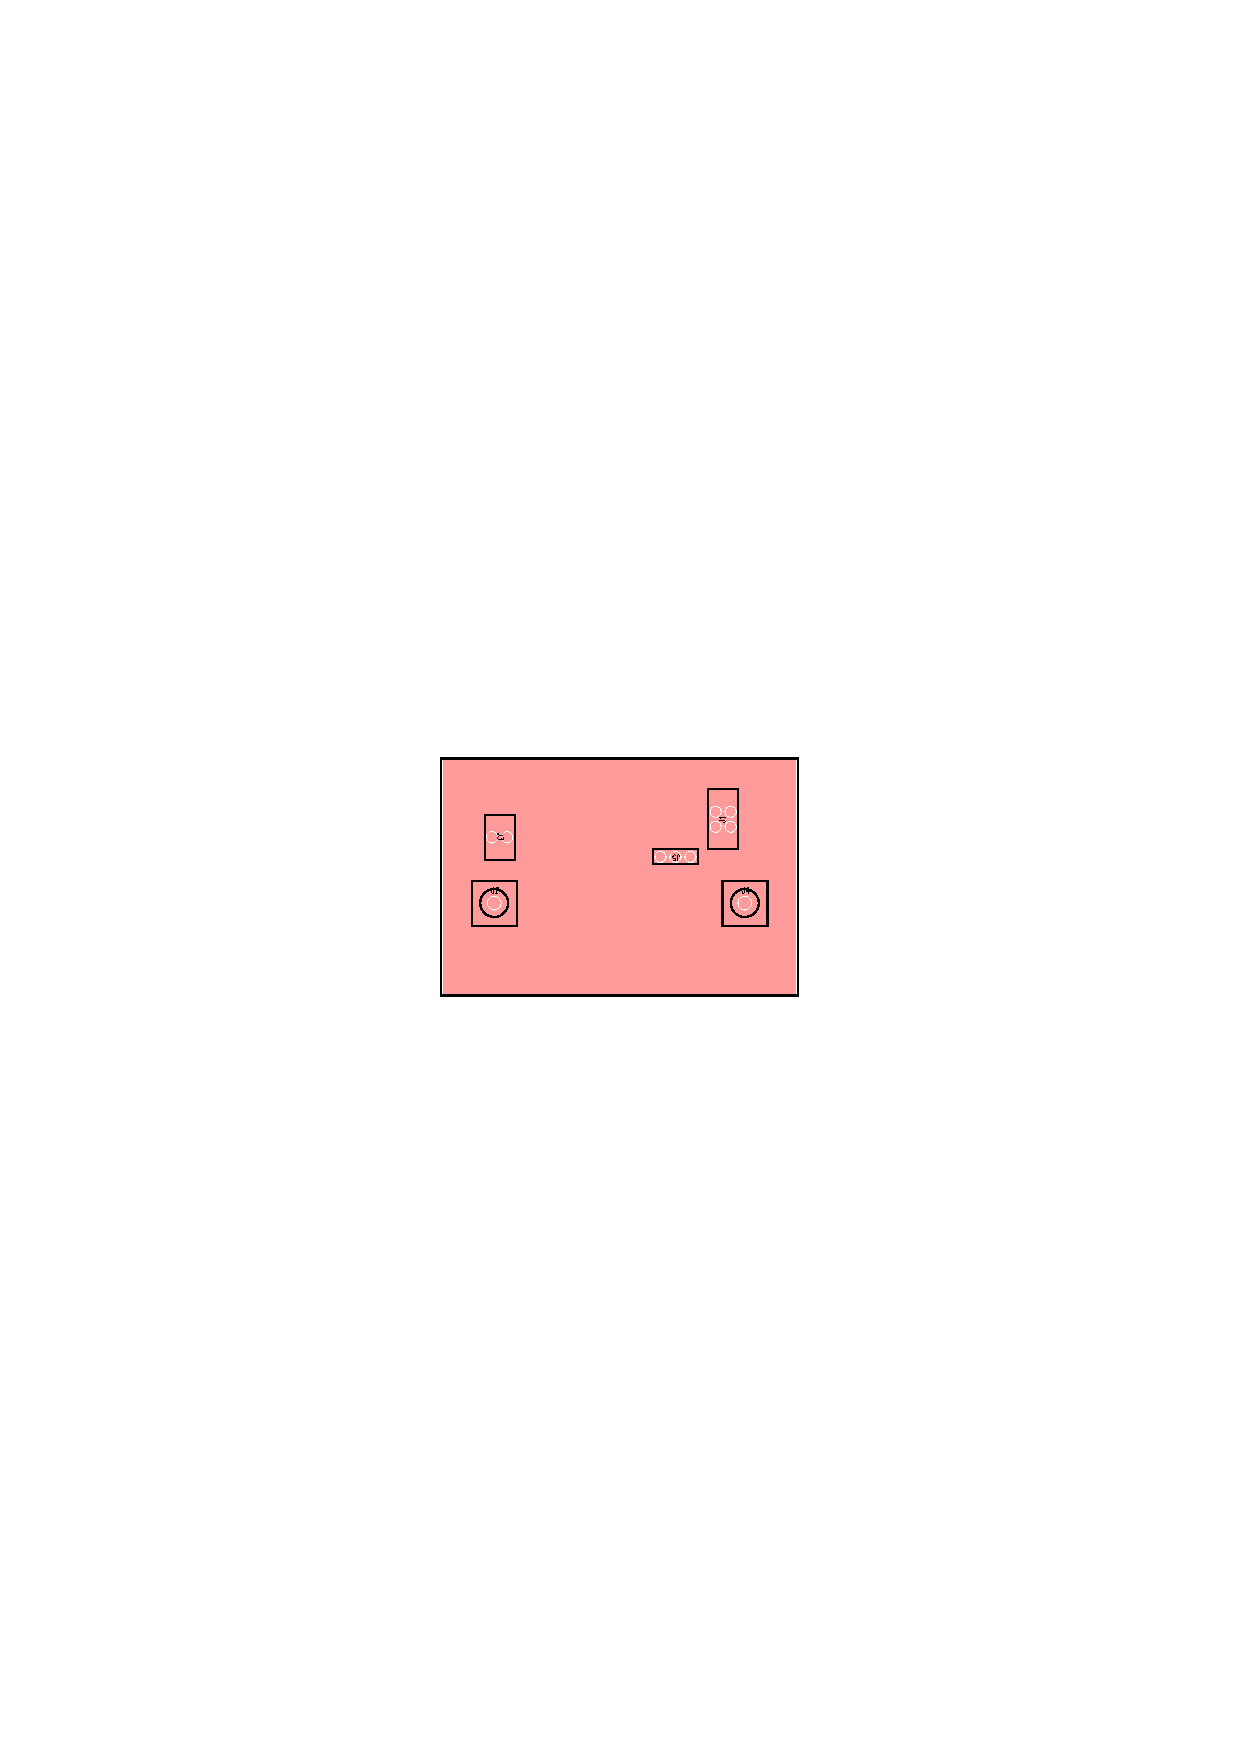
\includegraphics[trim = 7.3cm 12.7cm 7.3cm 12.7cm, clip, width=6.5cm]{../../CAM_DOC/O1.pdf}
  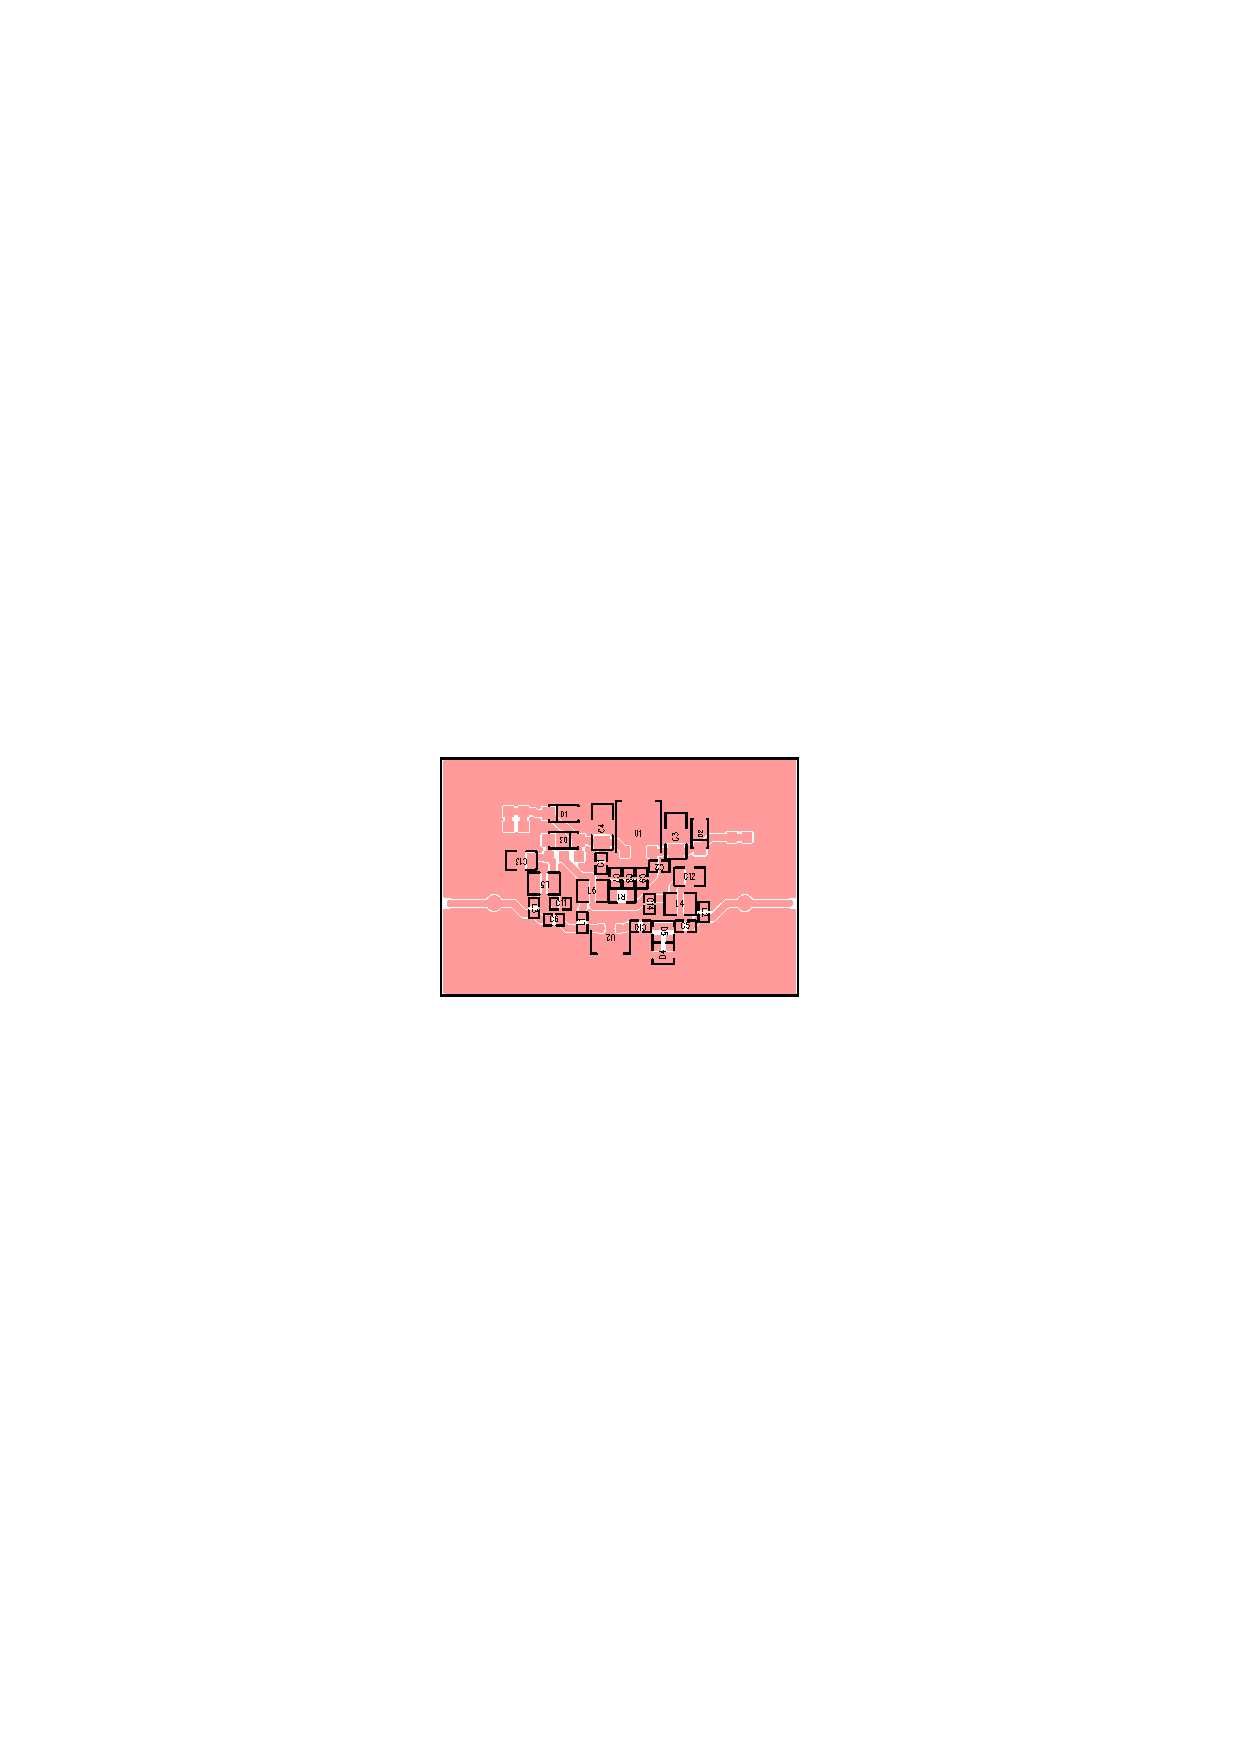
\includegraphics[trim = 7.3cm 12.7cm 7.3cm 12.7cm, clip, width=6.5cm]{../../CAM_DOC/O2.pdf}
  \caption{Osazovací plán horní a spodní strany plošného spoje}
  \label{fig:osazovaci_plan}
\end{figure}

\begin{savenotes}
\begin{table}[h!]
\begin{center}
\begin{tabular}{ |c|c|c|c| }
\hline 
Počet & Označení & Typ  & Pouzdro  \\ 
\hline 
7	&	C1,C2,C5,C6,C10,C11,C14	&	C0805	&	100nF	\\
2	&	C3,C4	&	ELYTC	&	47uF	\\
1	&	C7	&	C0805	&	68pF	\\
1	&	C8	&	C0805	&	1n2	\\
1	&	C9	&	C0805	&	1uF	\\
2	&	C12,C13	&	ELYTB	&	10uF/16V	\\
3	&	D1,D2,D3	&	SMA	&	M4	\\
2	&	D4,D5	&	SOT23	&	BAR43SSMD	\\
1	&	J1	&	JUMP2X4	&	JUMP2X4	\\
2	&	J2,J4	&	SMA6251A13G50	&	SMA6251A13G50	\\
1	&	J3	&	JUMP2X3	&	JUMP2X3	\\
1	&	J5	&	JUMP3	&	Power Bypass	\\
3	&	L1,L2,L3	&	R0805	&	MI0805K400R-10	\\
3	&	L4,L5,L6	&	L1812	&	CC453232-1R2KL	\\
1	&	R1	&	R1206	&	10R/0R	\\
1	&	U1	&	TO252	&	LM78M05CDT	\\
1	&	U2	&	SOT89	&	ADL5536	\\
\hline 
\end{tabular}
\end{center}
\caption{Seznam součástek pro všechny varianty osazení plošného spoje.}
\label{seznam_soucastek}
\end{table}
\end{savenotes}

\newpage

\subsubsection{Nastavení}
Nastavení modulu se provádí jumpery na jeho vrchní straně. 


\begin{thebibliography}{99}
\bibitem{Si570board}{Původní konstrukce Si570 Board } 
\href{http://wb6dhw.com/inactive.html}{http://wb6dhw.com/inactive.html}

\end{thebibliography}
\end{document}